% Chapter 2

\chapter{Intel PT背景知识}

\section{Intel PT简介}
英特尔处理器追踪(Intel Processor Trace,Intel PT)是Intel处理器结构的扩展,是一项最新的硬件功能,它使用专用的硬件设施捕获程序的运行时信息,只造成极小的额外开销。正确配置后,Intel PT追踪程序在CPU上的执行,收集控制流转移等相关信息,并对收集信息进行编码产生追踪数据。将记录的Intel PT追踪数据与程序二进制文件作为输入,软件解码器可以重新构建程序执行的精确控制流,图~\ref{fig:bigbigpicture}给出了利用Intel PT进行硬件Profiling的简要流程。

\begin{figure}[!htb]
  \centering
  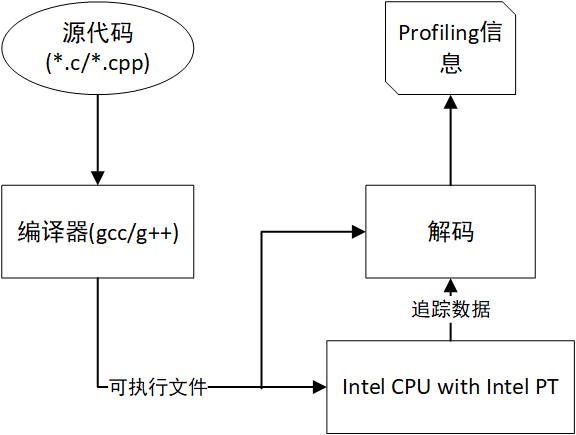
\includegraphics[width=0.8\textwidth]
  {figures/BIGBIGPicture.png}\\
  \caption{Intel PT硬件Profiling流程}
  \label{fig:bigbigpicture}
\end{figure}

Intel PT追踪数据由一系列的数据包组成,数据包能够记录控制流信息,例如间接分支目标的指令指针(IP)地址和条件分支方向(分支是否发生),除了控制流信息,数据包还记录了如上下文、时间戳等其他信息,从而可以对应用程序进行功能和性能调试。Intel PT具有多种形式的控制和过滤功能,可通过对特定的MSR寄存器编程进行配置,正确配置后能用于自定义收集的跟踪信息,并附加其他处理器状态和时序信息以启用调试。例如,有些模式允许基于当前特权级别(CPL)或CR3的值,以及指令指针地址的值对数据包进行过滤。\upcite{Intel}
为了解Intel PT如何启用控制流跟踪,表\ref{tab:1} 给出了主要的Intel PT生成数据包的类型、大小和功能:
\begin{table}[ht]
  \centering
  \caption{Intel PT数据包}
  \label{tab:1}
  \begin{tabular}{c|c|p{8cm}}
    \hline
    数据包& 大小(字节)& 功能\\
    \hline
    PSB& 16& Packet Stream Boundary,定期生成,充当数据包所构成的二进制流的边界,为解码器提供了一个同步点。\\
    \hline
    PGE& ≤8& Packet Generation Enable,标志着一段控制流追踪的开始,提供开始的指令指针地址\\
    \hline
    PGD& ≤8& Packet Generation Disable,标志着一段控制流追踪的结束,提供结束时指令指针地址\\
    \hline
    TNT& 1 or 8& Taken-Not-Taken,提供直接分支跳转的方向(发生或者未发生)\\
    \hline
    TIP& ≤8& Target Instruction Pointer,提供间接分支跳转、异常、中断等的目标指令指针地址\\
    \hline
    FUP& ≤8 &Flow Update Packet,提供无法异常、中断等无法推导源指令指针地址的异步事件的源指令指针地址\\
    \hline
    TSC& 8& Timestamp Counter,固定产生时钟周期计数值,和其他与时间相关的数据包一起能提供较准确的时间信息\\
    \hline
  \end{tabular}
\end{table}

Intel PT定期产生PSB数据包,标志着每段数据流的边界,为解码器提供了一个同步点,在解码时PSB数据包应该是解码器应该找的第一个数据包。Intel PT通过PGE和PGD数据包记录一段控制流追踪的开始和结束,在配置Intel PT时进行追踪时,可能添加了类似于当前用户权限(CPL),CR3寄存器,指令指针地址等过滤条件,当满足追踪条件时,会产生PGE数据包标志着一段控制流追踪的开始,当不满足时,则通过PGD标志一段控制流追踪的结束,但控制流追踪结束的情况,PT仍然有可能会产生时间、模式等相关的数据包。

为了压缩产生的信息,最小化生成数据包的大小,Intel PT对不同的分支指令采用了不同的方式记录,对于JMP (E9 xx, EB xx), CALL (E8 xx)等无条件跳转指令,它们的目标地址嵌入在指令中,目标地址可以直接从二进制文件中推导,Intel PT忽略了此类跳转信息的记录,对于条件分支指令(JCC, J*CXZ) 和LOOP指令,Intel PT使用TNT数据包中的一个比特记录了分支的方向(发生/未发生),1个字节的TNT数据包最多能记录6个条件分支,8个字节的TNT数据包最多能记录47个条件分支,对于类似于JMP (FF /4), CALL (FF /2) 等间接分支指令和RET (C3, C2 xx)等返回指令,Intel PT用TIP数据包记录了目标指令指针地址,为了减小TIP数据包的大小,如果高位地址字节与先前记录的地址匹配,则英特尔PT压缩目标地址,最多可压缩六个字节,此外,对于RET指令,若目标地址与先前的调用匹配,Intel PT将其压缩为TNT的一位。对于中断、异常等异步事件指令,Intel PT除了用TIP数据包记录了目标指令指针地址,还用FUP数据包记录了发生此事件的源指令指针地址。Intel PT的数据包压缩机制会导致数据包之间存在依赖关系,这对并行化的处理提出了挑战。

Intel PT的输出机制独立于追踪和过滤机制,输出选项可能随处理器和平台的不同而变化。Intel PT将追踪数据包直接输出到物理内存中,绕过缓存和TLB以减少对程序性能造成的影响,目前内存配置有三种方式:1. 物理地址空间的单一连续区域;2. 可以通过使用类似于表的数据结构来配置使用物理地址空间中不连续的多个缓冲区,当缓冲区已满,可以触发中断;3. Intel PT支持一种特定于平台的子系统输出机制。

Intel PT支持所选进程/线程的用户空间和内核空间的追踪,通过相应的配置后,能够仅追踪特定的进程/线程在用户空间/内核空间的执行,在本课题中实现C/C++程序的Profiling时,我们更关注对某一进程的用户空间执行的追踪。

\section{{Intel PT追踪配置}}
Intel PT追踪数据包的生成通过特定于模型的寄存器(MSR)集合来启用和配置,目前在Linux系统上提供Intel PT追踪实现获取数据的工具主要有:

1. simple-PT是Intel PT在Linux系统上的简单实现,它支持使用备用的内核驱动程序在Linux上捕获Intel PT,使得Intel PT能以适度的开销追踪CPU在硬件级别执行的控制流。 该项目包括一个配置Intel PT的内核驱动模块,一个导出PT数据的模块,一个能显示函数、指令级追踪的解码模块、一个仅显示PT数据包的快速解码模块。不过simple-PT不支持中断,不能够长期导出PT数据,当追踪生成的PT数据超过为其所配置的内存时,将会丢失。\upcite{simple-pt}

2. 从4.1版开始,Linux内核通过perf event内核接口支持对Intel PT的配置追踪。 从4.3版开始,用户空间Profiling工具perf也支持Intel PT,perf通过调用perf event内核接口实现对Intel PT的配置,支持两种模式下的追踪:Full Trace模式下,perf会连续向磁盘中导出追踪过程中的全部PT数据,Snapshot模式下,生成的PT数据会不断向内存中重写,直到停止追踪,并只导出追踪结束前的数据,这种模式对软件的调试有重要的帮助。\upcite{perf-event-open}

3. 除此以外,Intel的Profiling工具VTune\upcite{Vtune}提供了对Intel PT的支持,它具有较为强大的功能支持;gdb\upcite{GDB}从7.10开始的版本通过利用perf event内核接口也提供了对Intel PT的支持,很好地实现了进程的记录和重放,在断点或故障时,能够很容易的看到之前的指令流,在利用gdb进行调试时有很好的效果。

为了使追踪模块更简洁且易于控制,本课题主要利用了perf event内核接口实现了简单的Intel PT的追踪配置和数据导出。

下面具体介绍了perf event内核接口的配置方式:perf event open内核接口提供了在Linux用户态建立性能监控的途径,指定参数后,系统调用perf\_event\_open返回一个文件描述符,每一个文件描述符对应一项被监控的系统事件,多个文件描述的组合可用来监控多种事件,此文件描述符可以被以后的系统调用(ioctl, prctl, read, mmap等)所使用。ioctl、prctl系统调用控制事件的启用或禁用,事件分为两种形式,计数事件通过系统调用read访问,采样事件通过系统调用mmap配置采样结果在内存的写入和访问。参数列表中参数pid和cpu指定了监控某个进程/线程和cpu的事件,group\_fd允许创建一个事件组,首先创建的事件该参数为-1,该组的其他事件指定group\_fd为首先创建事件的返回值。参数flags指定了该事件的部分标识,包括是否支持系统级监控、是否忽略group\_fd等。参数attr具体配置了事件的相关信息,包括事件类型、该类型事件的具体配置、是否监控用户空间、是否监控内核空间等。

为了配置Intel PT追踪进程在用户空间的执行,我们主要需要进行两个方面的配置:

1.Intel PT事件,通过读取Linux下的/sys/bus/event\_source/devices/intel\_pt/type文件可以获取Intel PT的动态PMU值,根据需要,具体配置PT事件相关的attr参数信息,然后对所期望追踪的进程和每一个CPU进行监控,通过mmap系统调用设置每一个CPU产生PT追踪数据的内存,通过ioctl系统调用控制事件的启动和禁用。

2.为了对Intel PT进行解码,除了需要配置Intel PT相关的事件,我们还需要实现对其他信息的记录,例如二进制文件的加载(需要将某个时刻的PT记录信息与其记录执行的二进制文件对应),线程切换信息(为了得到当前执行的线程信息,获得对多线程的支持)等。首先配置监控事件的类型为PERF\_TYPE\_SOFTWARE,具体配置所需相关事件的attr相关信息,同样需要监控对预期追踪的进程以及每一个CPU进行监控,利用mmap系统调用设置该事件产生结果写入的内存,利用ioctl控制事件的启动和禁用。

\iffalse
\section{Intel PT顺序解码过程}
以表\ref{tab:2}为例(程序流以基本块为单位,仅显示了控制流转移相关的指令),此节在较高的层面给出利用Intel PT追踪数据顺序解码的流程。

Intel PT顺序解码的流程较为清晰,然而由于追踪过程中产生的大量数据包,使得解码的开销经常很高,是追踪过程开销的2到3个数量级,因此本课题研究的主要目的在于减少解码阶段的开销,主要通过考虑实现解码阶段的并行化解码,然而Intel PT数据包存在的顺序依赖关系使得PT数据的划分并不能随意进行,因此为实现解码阶段的并行化,如何更好的解决Intel PT数据包存在的顺序依赖关系,实现较好的数据划分,从而对划分后的数据进行并行化的解码是本课题需要解决的重要问题。
\begin{table}[ht]
  \centering
  \caption{}
  \label{tab:2}
  \begin{tabular}{|p{4cm}|p{6cm}|}
    \hline
    A:…& PGE(A)\\
    \quad jmp D& TNT: 1 | 0 | End\\
    B:…& TIP(F)\\
    \quad jcc E& PGD(F)\\
    C:…&\\
    \quad Call *eax&\\
    D:…&\\
    \quad jcc B&\\
    E: …&\\
    \quad ret&\\
    \hline
  \end{tabular}
\end{table}
\fi